\documentclass[11pt]{article}

% Increase main memory size
\usepackage{etex}
\usepackage{morewrites}
\usepackage{multicol}
\usepackage{pgfplots}
\usepackage{tikz}
\usetikzlibrary{external}
\tikzexternalize[prefix=cached_models/]
% Ensure the directory exists
\immediate\write18{mkdir -p cached_models}

\usepackage{etex}
\usepackage{morewrites}
\usepackage{enumitem}
\usepackage{float}

\listfiles

\usepackage{amsmath, amssymb, amsthm}
\usepackage{graphicx}
\usepackage{geometry}
\usepackage{array}
\usepackage{booktabs}
\usepackage{float}
\usepackage{verbatim}
\usetikzlibrary{3d}

% Page Layout
\geometry{a4paper, margin=1in}
\setlength\parindent{0pt}
\pgfplotsset{compat=1.18}

% Custom commands
\newcommand{\card}[1]{\lvert #1 \rvert}
\newcommand{\inner}[2]{\left\langle #1, #2 \right\rangle}

\title{\textbf{Principles of Mathematical Analysis}}
\author{}
\date{}

\begin{document}

\maketitle

\section{Measure Theory}
\subsection{Riemann Integral}
For a bounded function \( f: [a, b] \to \mathbb{R} \) and any partition of the interval \([a, b]\), \(P = \{a = x_0 < x_1 < \ldots < x_n = b\}\), we consider on each subinterval \(I_j = [x_{j-1}, x_j], \quad j = 1, \ldots, n\), the quantities:
\[M_j = \sup_{x \in I_j} f(x), \quad m_j = \inf_{x \in I_j} f(x).\]

We also define the upper and lower sums of \(f\) with respect to the partition \(P\) as:
\[U_f(P) = \sum_{j=1}^{n} M_j (x_j - x_{j-1}), \quad L_f(P) = \sum_{j=1}^{n} m_j (x_j - x_{j-1}).\]

\begin{center}
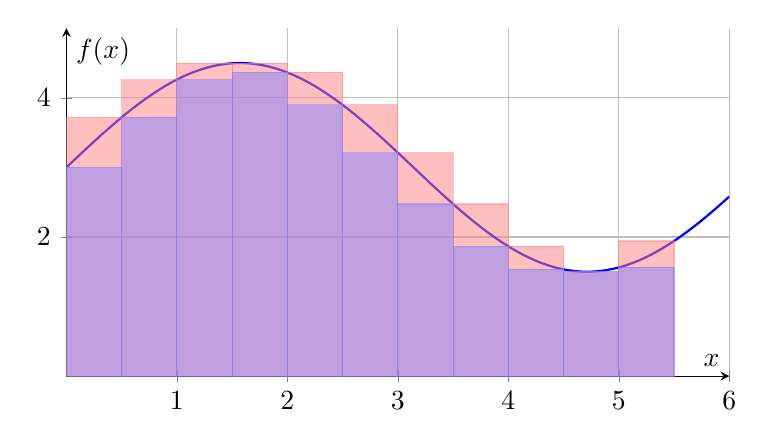
\begin{tikzpicture}
    \begin{axis}[
        axis lines = middle,
        xlabel = \(x\),
        ylabel = {\(f(x)\)},
        domain=0:6,
        samples=100,
        ymin=0, ymax=5,
        xmin=0, xmax=6,
        width=10cm,
        height=6cm,
        grid=both,
    ]
    \addplot[blue, thick] {1.5*sin(deg(x)) + 3};
    \addplot[red!50, fill=red!50, opacity=0.5] coordinates {(0,0) (0,{1.5*sin(deg(0.5))+3}) (0.5,{1.5*sin(deg(0.5))+3}) (0.5,0)} -- cycle;
    \addplot[red!50, fill=red!50, opacity=0.5] coordinates {(0.5,0) (0.5,{1.5*sin(deg(1))+3}) (1,{1.5*sin(deg(1))+3}) (1,0)} -- cycle;
    \addplot[red!50, fill=red!50, opacity=0.5] coordinates {(1,0) (1,{1.5*sin(deg(1.5))+3}) (1.5,{1.5*sin(deg(1.5))+3}) (1.5,0)} -- cycle;
    \addplot[red!50, fill=red!50, opacity=0.5] coordinates {(1.5,0) (1.5,{1.5*sin(deg(1.5))+3}) (2,{1.5*sin(deg(1.5))+3}) (2,0)} -- cycle;
    \addplot[red!50, fill=red!50, opacity=0.5] coordinates {(2,0) (2,{1.5*sin(deg(2))+3}) (2.5,{1.5*sin(deg(2))+3}) (2.5,0)} -- cycle;
    \addplot[red!50, fill=red!50, opacity=0.5] coordinates {(2.5,0) (2.5,{1.5*sin(deg(2.5))+3}) (3,{1.5*sin(deg(2.5))+3}) (3,0)} -- cycle;
    \addplot[red!50, fill=red!50, opacity=0.5] coordinates {(3,0) (3,{1.5*sin(deg(3))+3}) (3.5,{1.5*sin(deg(3))+3}) (3.5,0)} -- cycle;
    \addplot[red!50, fill=red!50, opacity=0.5] coordinates {(3.5,0) (3.5,{1.5*sin(deg(3.5))+3}) (4,{1.5*sin(deg(3.5))+3}) (4,0)} -- cycle;
    \addplot[red!50, fill=red!50, opacity=0.5] coordinates {(4,0) (4,{1.5*sin(deg(4))+3}) (4.5,{1.5*sin(deg(4))+3}) (4.5,0)} -- cycle;
    \addplot[red!50, fill=red!50, opacity=0.5] coordinates {(4.5,0) (4.5,{1.5*sin(deg(4.66))+3}) (5,{1.5*sin(deg(4.66))+3}) (5,0)} -- cycle;
    \addplot[red!50, fill=red!50, opacity=0.5] coordinates {(5,0) (5,{1.5*sin(deg(5.5))+3}) (5.5,{1.5*sin(deg(5.5))+3}) (5.5,0)} -- cycle;

    \addplot[blue!50, fill=blue!50, opacity=0.5] coordinates {(0,0) (0,{1.5*sin(deg(0))+3}) (0.5,{1.5*sin(deg(0))+3}) (0.5,0)} -- cycle;
    \addplot[blue!50, fill=blue!50, opacity=0.5] coordinates {(0.5,0) (0.5,{1.5*sin(deg(0.5))+3}) (1,{1.5*sin(deg(0.5))+3}) (1,0)} -- cycle;
    \addplot[blue!50, fill=blue!50, opacity=0.5] coordinates {(1,0) (1,{1.5*sin(deg(1))+3}) (1.5,{1.5*sin(deg(1))+3}) (1.5,0)} -- cycle;
    \addplot[blue!50, fill=blue!50, opacity=0.5] coordinates {(1.5,0) (1.5,{1.5*sin(deg(2))+3}) (2,{1.5*sin(deg(2))+3}) (2,0)} -- cycle;
    \addplot[blue!50, fill=blue!50, opacity=0.5] coordinates {(2,0) (2,{1.5*sin(deg(2.5))+3}) (2.5,{1.5*sin(deg(2.5))+3}) (2.5,0)} -- cycle;
    \addplot[blue!50, fill=blue!50, opacity=0.5] coordinates {(2.5,0) (2.5,{1.5*sin(deg(3))+3}) (3,{1.5*sin(deg(3))+3}) (3,0)} -- cycle;
    \addplot[blue!50, fill=blue!50, opacity=0.5] coordinates {(3,0) (3,{1.5*sin(deg(3.5))+3}) (3.5,{1.5*sin(deg(3.5))+3}) (3.5,0)} -- cycle;
    \addplot[blue!50, fill=blue!50, opacity=0.5] coordinates {(3.5,0) (3.5,{1.5*sin(deg(4))+3}) (4,{1.5*sin(deg(4))+3}) (4,0)} -- cycle;
    \addplot[blue!50, fill=blue!50, opacity=0.5] coordinates {(4,0) (4,{1.5*sin(deg(4.5))+3}) (4.5,{1.5*sin(deg(4.5))+3}) (4.5,0)} -- cycle;
    \addplot[blue!50, fill=blue!50, opacity=0.5] coordinates {(4.5,0) (4.5,{1.5*sin(deg(4.66))+3}) (5,{1.5*sin(deg(4.66))+3}) (5,0)} -- cycle;
    \addplot[blue!50, fill=blue!50, opacity=0.5] coordinates {(5,0) (5,{1.5*sin(deg(5))+3}) (5.5,{1.5*sin(deg(5))+3}) (5.5,0)} -- cycle;
    \end{axis}
\end{tikzpicture}
\end{center}

For any two partitions \(P\) and \(Q\) of \([a, b]\), we have:
\[L_f(P) \leq \text{Area under } f \leq U_f(Q).\]

If $P$ has a value $I$ such that:
\[\sup_{P} L_f(P) = I = \inf_{P} U_f(P),\]
then we say that \(f\) is Riemann integrable on \([a, b]\) and define the Riemann integral of \(f\) over \([a, b]\) as:
\[\int_a^b f(x) \, dx = I.\]

Continuous functions on closed intervals are Riemann integrable.
\subsection{The Lebesgue Integral}
A bounded function \( f: [a, b] \to \mathbb{R} \) is said to be \textit{Lebesgue integrable} on \([a, b]\) if the set of points where \(f\) is discontinuous has zero measure. 

A set $B \subset \mathbb{R}$ has \textit{measure zero} if for every $\epsilon > 0$, it can be covered by a countable collection of open intervals $\{(a_n, b_n)\}$ such that:
\[B \subset \bigcup_{n=1}^{\infty} (a_n, b_n) \quad \text{and} \quad \sum_{n=1}^{\infty} (b_n - a_n) < \epsilon.\]

\subsubsection{Example: Dirichlet Function}
The Dirichlet function:
\[ f(x) = \chi_{\mathbb{Q}}(x) = \begin{cases} 1 & \text{if } x \in \mathbb{Q}, \\ 0 & \text{if } x \notin \mathbb{Q}, \end{cases} \]

On the interval \([0, 1]\): 
\begin{center}
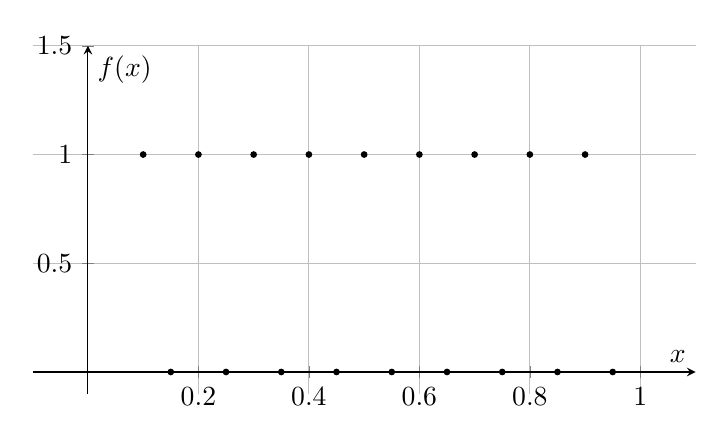
\begin{tikzpicture}
    \begin{axis}[
        axis lines = middle,
        xlabel = \(x\),
        ylabel = {\(f(x)\)},
        domain=0:1,
        samples=100,
        ymin=-0.1, ymax=1.5,
        xmin=-0.1, xmax=1.1,
        width=10cm,
        height=6cm,
        grid=both,
    ]
    \addplot[only marks, mark=*, mark size=1pt] coordinates {
        (0.1,1) (0.2,1) (0.3,1) (0.4,1) (0.5,1) (0.6,1) (0.7,1) (0.8,1) (0.9,1)
        (0.15,0) (0.25,0) (0.35,0) (0.45,0) (0.55,0) (0.65,0) (0.75,0) (0.85,0) (0.95,0)
    };
    \end{axis}
\end{tikzpicture}
\end{center}

We see that \(f\) is not Riemann integrable since it is discontinuous everywhere. 

But consider, 
\[\mathbb{Q} = \{q_1, q_2, q_3, \ldots\}\] 
and define:
\[f_1(x) = \chi_{\{q_1\}}(x) \rightarrow \text{integrable on } [0, 1]\]
\[f_2(x) = \chi_{\{q_1, q_2\}}(x) \rightarrow \text{integrable on } [0, 1]\]
\[\vdots\]
\[f_n(x) = \chi_{\{q_1, q_2, \ldots, q_n\}}(x) \rightarrow \text{integrable on } [0, 1]\]

Then,
\[\lim_{n \to \infty} f_n(x) = \chi_{\mathbb{Q}}(x).\]

\subsubsection{Characteristic Function}
For any set \(A \subset \mathbb{R}\), the characteristic function \(\chi_A: \mathbb{R} \to \{0, 1\}\) is defined as:
\[\chi_A(x) = \begin{cases} 1 & \text{if } x \in A, \\ 0 & \text{if } x \notin A. \end{cases}\]

\[\int_0^1 f_1(x) \, dx = 0 = \int_0^1 f_2(x) \, dx = \ldots = \int_0^1 f_n(x) \, dx = 0.\]

\subsubsection*{Example}
Let 
\[f_n(x) = \begin{cases} x^n & \text{if } 0 \leq x < 1, \\ 0 & \text{if } 1 \leq x. \end{cases}\]

Then, with $f_n(x)$ continuous on $\mathbb{R}$, we have:

\[\lim_{n \to \infty} f_n(x) = \begin{cases} 0 & \text{if } 0 \leq x < 1, \\ 1 & \text{if } x \leq 1. \end{cases}\]

so we can see that there is a discontinuity at \(x = 1\).

\begin{center}
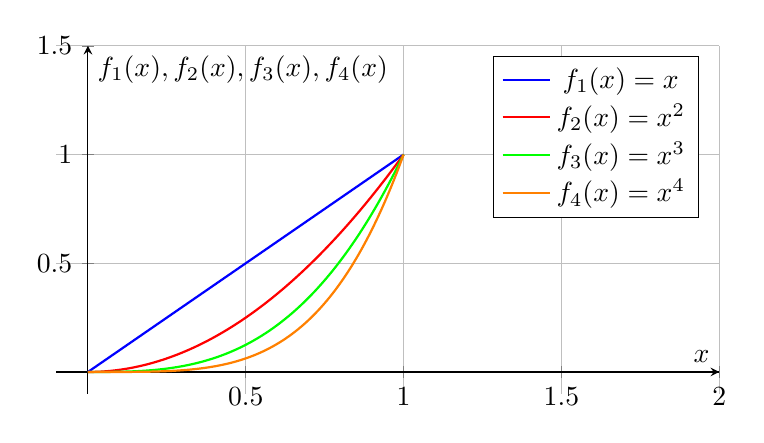
\begin{tikzpicture}
    \begin{axis}[
        axis lines = middle,
        xlabel = \(x\),
        ylabel = {\(f_1(x), f_2(x), f_3(x), f_4(x)\)},
        domain=0:1,
        samples=100,
        ymin=-0.1, ymax=1.5,
        xmin=-0.1, xmax=2,
        width=10cm,
        height=6cm,
        grid=both,
        legend pos=north east
    ]
    \addplot[blue, thick] {x};
    \addlegendentry{\(f_1(x) = x\)}

    \addplot[red, thick] {x^2};
    \addlegendentry{\(f_2(x) = x^2\)}

    \addplot[green, thick] {x^3};
    \addlegendentry{\(f_3(x) = x^3\)}

    \addplot[orange, thick] {x^4};
    \addlegendentry{\(f_4(x) = x^4\)}

    \addplot[black, thick] coordinates {(1,0) (2,0)};
    \end{axis}
\end{tikzpicture}
\end{center}

\subsubsection*{Example}
Let
\[f_n(x) = \begin{cases} -1 & \text{if } x \leq -\frac{1}{n}, \\ \sin\left(\dfrac{n\pi x}{2}\right) & \text{if } -\frac{1}{n} \leq x \leq \frac{1}{n}, \\ 1 & \text{if } \frac{1}{n} \leq x. \end{cases}\]

Then, with $f_n(x)$ continuous and differentiable on $\mathbb{R}$, we have:
\[\lim_{n \to \infty} f_n(x) = \begin{cases} -1 & \text{if } x < 0, \\ 0 & \text{if } x = 0, \\ 1 & \text{if } x > 0. \end{cases}\]
\begin{center}
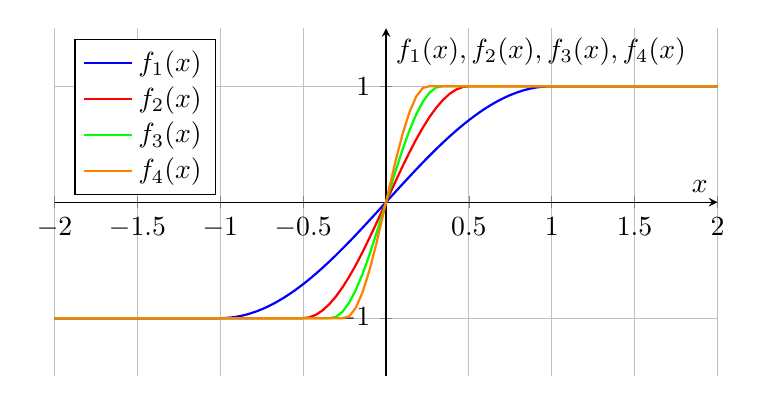
\begin{tikzpicture}
    \begin{axis}[
        axis lines = middle,
        xlabel = \(x\),
        ylabel = {\(f_1(x), f_2(x), f_3(x), f_4(x)\)},
        domain=-2:2,
        samples=100,
        ymin=-1.5, ymax=1.5,
        xmin=-2, xmax=2,
        width=10cm,
        height=6cm,
        grid=both,
        legend pos=north west
    ]
    \addplot[blue, thick] {x <= -1 ? -1 : (x >= 1 ? 1 : sin(deg(pi*x/2)))};
    \addlegendentry{\(f_1(x)\)}

    \addplot[red, thick] {x <= -0.5 ? -1 : (x >= 0.5 ? 1 : sin(deg(2*pi*x/2)))};
    \addlegendentry{\(f_2(x)\)}

    \addplot[green, thick] {x <= -0.33 ? -1 : (x >= 0.33 ? 1 : sin(deg(3*pi*x/2)))};
    \addlegendentry{\(f_3(x)\)}

    \addplot[orange, thick] {x <= -0.25 ? -1 : (x >= 0.25 ? 1 : sin(deg(4*pi*x/2)))};
    \addlegendentry{\(f_4(x)\)}
    \end{axis}
\end{tikzpicture}
\end{center}

\subsubsection*{Example}
The Dirichlet function is not integrable but it is the limit of a sequence of integrable functions, all with integral equal to zero.

We need to define a new kind of convergence.

\subsection{Convergences}
A sequence of functions \(\{f_n\}_{n \in \mathbb{N}}\) converges punctually to a function \(f\) on \(Dom(f)\) if:
\[\lim_{n \to \infty} f_n(x) = f(x), \quad \forall x \in Dom(f).\]

\[\forall \epsilon > 0, \quad \forall x \in Dom(f), \quad \exists N (\epsilon, x) \in \mathbb{N} : n > N \implies |f_n(x) - f(x)| < \epsilon.\]

A sequence of functions \(\{f_n\}_{n \in \mathbb{N}}\) converges uniformly to a function \(f\) on \(Dom(f)\) if:
\[\forall \epsilon, \quad \exists N : n > N \implies |f_n(x) - f(x)| < \epsilon, \quad \forall x \in Dom(f).\]

\subsubsection*{Example}
Let
\[f_n(x) = \frac{1}{n} \sin(nx), \quad x \in \mathbb{R}. \rightarrow^{n\to\infty} f(x) = 0.\]

\begin{center}
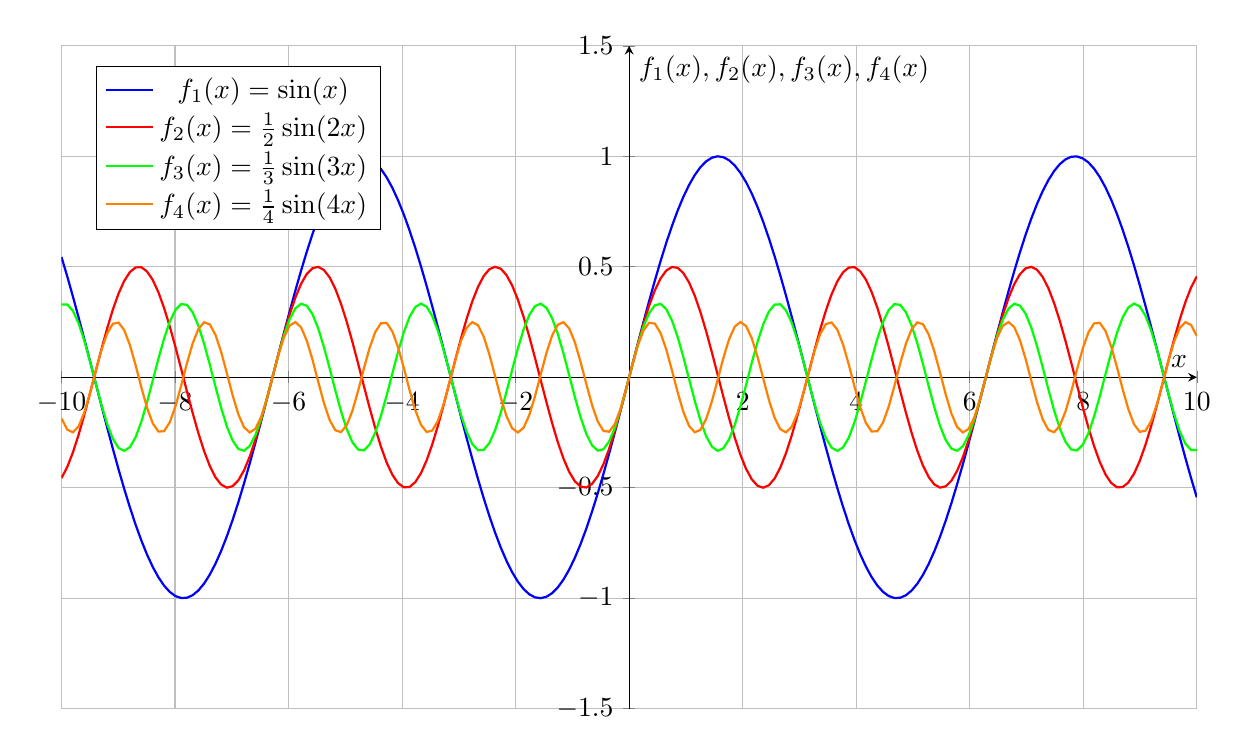
\begin{tikzpicture}
    \begin{axis}[
        axis lines = middle,
        xlabel = \(x\),
        ylabel = {\(f_1(x), f_2(x), f_3(x), f_4(x)\)},
        domain=-10:10,
        samples=200,
        ymin=-1.5, ymax=1.5,
        xmin=-10, xmax=10,
        width=16cm,
        height=10cm,
        grid=both,
        legend pos=north west
    ]
    \addplot[blue, thick] {1*sin(deg(x))};
    \addlegendentry{\(f_1(x) = \sin(x)\)}

    \addplot[red, thick] {1/2*sin(deg(2*x))};
    \addlegendentry{\(f_2(x) = \frac{1}{2}\sin(2x)\)}

    \addplot[green, thick] {1/3*sin(deg(3*x))};
    \addlegendentry{\(f_3(x) = \frac{1}{3}\sin(3x)\)}

    \addplot[orange, thick] {1/4*sin(deg(4*x))};
    \addlegendentry{\(f_4(x) = \frac{1}{4}\sin(4x)\)}
    \end{axis}
\end{tikzpicture}
\end{center}

\subsubsection{Uniform Convergence}
\begin{enumerate}
    \item If \(\{f_n\}_{n \in \mathbb{N}}\) converges uniformly to \(f\) on \([a, b]\) and each \(f_n\) is continuous, then:
        \[\int_a^b f(x) \, dx = \lim_{n \to \infty} \int_a^b f_n(x) \, dx.\]
    \item If \(\{f_n\}_{n \in \mathbb{N}}\) converges uniformly to \(f\) on \([a, b]\) and each \(f_n\) is continuous in \([a, b]\), then \(f\) is continuous on \([a, b]\).
    \item If \(\{f_n\}_{n \in \mathbb{N}}\) is a sequence of differentiable functions on \([a, b]\) that converges punctually to some continuous function \(f\) on \([a, b]\) and if the sequence of derivatives \(\{f_n'\}_{n \in \mathbb{N}}\) converges uniformly to some continuous function \(g\), then \(f\) is differentiable on \((a, b)\) and:
        \[f'(x) = g(x) = \lim_{n \to \infty} f_n'(x).\]
\end{enumerate}

\subsection{Henri Lebesgue (1875-1941)}
How can we count money in bills?
\begin{enumerate}
    \item Add each amount as the bills come in. (Riemann)
    \item Make groups by denomination and count each group. (Lebesgue)
\end{enumerate}

\end{document}